% \section{Démarche Expérimentale}

\begin{wrapfigure}{R}{0.6\linewidth}
    \vspace{-1cm}
    \centering
    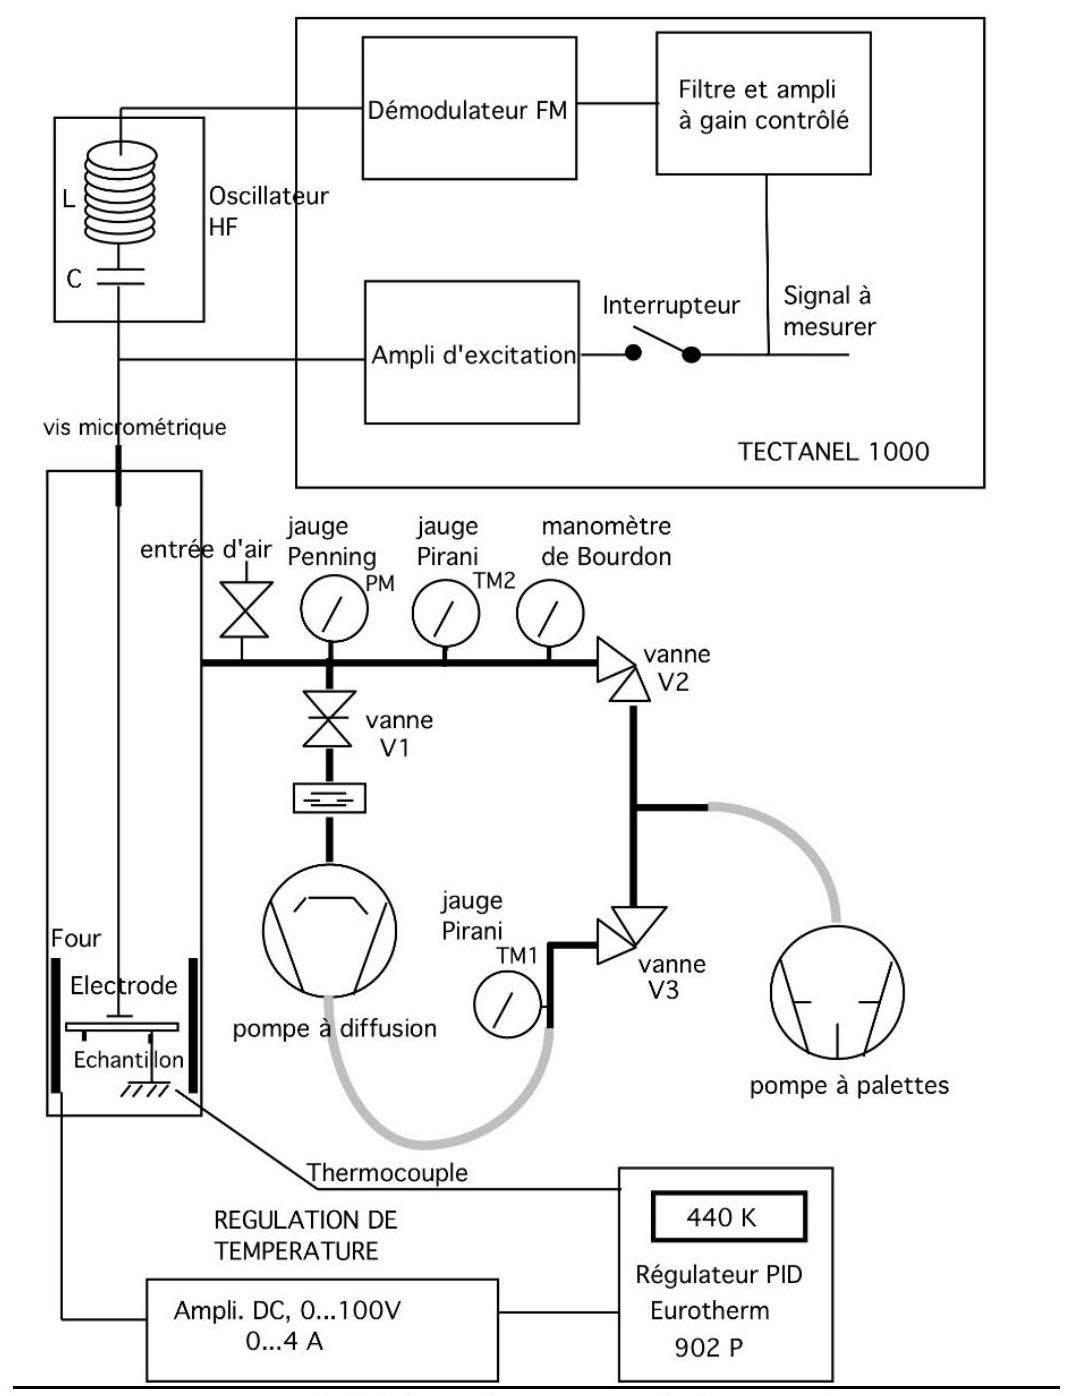
\includegraphics[width=\linewidth]{figures/montage.png}
    \caption{Montage expérimental \cite{notice}}
    \label{fig:montage}
    \vspace{-1cm}
\end{wrapfigure}

\paragraph{Démarche} Les mesures sont réalisées à l'aide du montage en \autoref{fig:montage}. Afin de limiter les frottements entre l'air et l'échantillon, l'installation est placée sous vide. L'échantillon est alors stimulé et vibre, avec une amplitude est mesurée grâce à l'électrode. Un programme informatique permet alors d'obtenir la fréquence des oscillations et de calculer le module de Young \(E\) avec
\begin{equation}
    E = 0.934 \frac{\rho L^4}{e^2}f^2
    \label{eq:young_programme}
\end{equation}
où \(\rho\) est la masse volumique de l'échantillon, \(L\) sa longueur, \(e\) son épaisseur et \(f\) la fréquence fondamentale de vibration. Le programme calcule aussi la capacité d'amortissement \(Q^{-1}\), à partir de l'amplitude des oscillations lors de la décroissance libre des oscillations, en utilisation l'equation
\begin{equation}
    Q^{-1} = \frac{1}{n \pi} \ln \frac{A_i}{A_{i+n}}
    \label{eq:q1_programme}
\end{equation}
avec \(A_i\) et \(A_{i+n}\) l'amplitude du \(i\)-ème et \(i+n\)-ième pic.

Afin d'observer les propriétés de l'échantillon, plus précisément le module de Young et la capacité d'amortissement, en fonction de la température, un régulateur PID permet de controler la chauffage progressif de l'échantillon.
